\documentclass[12pt]{amsart}
\usepackage{a4}
\usepackage{amsmath,amssymb,amsthm}
\usepackage{multicol}
\usepackage{verbatim}
\usepackage{graphicx, subfigure}
\newcommand{\sgn}{\mathop{\mathrm{sgn}}}
\newcommand{\ignore}[1]{}
\newcommand{\mat}[4]{\left(\begin{array}{ccc} #1 & #2 \\#3 & #4 \end{array} \right)}
\newcommand{\vect}[2]{\left(\begin{array}{ccc} #1 \\#2 \end{array} \right)}
\newcommand{\matc}[9]{\left(\begin{array}{ccc} #1 & #2 & #3 \\#4 & #5 & #6 \\#7 & #8 & #9 \end{array} \right)}
\begin{document}

\title{Overview}
\maketitle

I am writing a graphics program to visualize three-dimensional non-Euclidean geometry, with emphasis on connected sums of manifolds.

Currently, I have implemented $\mathbb{E}^3$, $\mathbb{H}^3$ and a space homeomorphic to $S^2 \times \mathbb{R}$.

I am in the process of implementing a method to glue multiple spaces together along spherical boundaries.

Outside Euclidean geometry, gluing spaces together like this won't always be smooth. More precisely, since two spheres with the same surface area do not generally have the same curvature, gluing the spaces together by those spheres will result in them having different curvature from each side. A similar problem will occur if the insides or outsides of two spheres are glued together.

In order to address this problem, I have designed and am currently in the process of implementing what I call wormhole.

I define an $(n,m)$-surface of revolution as an $(n+m)$-manifold with an automorphism group that has the automorphism group of the $n$-sphere as a subgroup. An $(n,m)$-surface of revolution is also an $(n-1,m+1)$-surface of revolution for all $n \geq 1$. In addition, this definition is based entirely upon the intrinsic geometry of the space, and does not require embedding into Euclidean geometry.

%A $2$-wormhole is a $(1,1)$-surface of revolution of constant negative Gaussian curvature. This makes it a quotient space on $\mathbb{H}^2$, for which it is easy to find geodesics.

I define a $2$-wormhole as a quotient space on $\mathbb{H}^2$ made by identifying two ultraparallel lines. This is a $(1,1)$-surface of revolution.

An $n$-wormhole is an $(n-1,1)$-surface of revolution. Generally, this does not have constant curvature, and is not a quotient space on $\mathbb{H}^n$. However, I have found a method to reduce finding a geodesic on an $(n,m)$-surface of revolution to a $(1,m)$-surface of revolution. In particular, I can find the geodesic on an $n$-wormhole using the method to find a geodesic on a $2$-wormhole.

There are two other spaces that are similar to this wormhole that are of interest. I hope to program these, but they are not part of my main goal. If I run out of time, I will consider the project complete without them. I call one a black hole and the other a cone point space. These spaces, and the wormhole, all are built by extending to the third dimension a quotient space of $\mathbb{H}^2$ in which two lines are identified. The wormhole occurs if the two lines are ultraparallel, the black hole if they're asymptotic, and the cone point space if they intersect.

Black holes and cone spaces can support the connection of two spaces in a similar manner, but they're more interesting just connected to one. \ignore{Why?} An $n$-black hole is an $n$-dimensional analogue of a pseudosphere, in which the embedding into $\mathbb{E}^3$ which has spherical cross-sections instead of circular ones. An $n$-cone point space is notable for containing a cone point and still being easy to connect to $\mathbb{E}^n$ or $\mathbb{H}^n$.

Another way to generalize this is to identify lines on $\mathbb{E}^2$ or $S^2$ instead of $\mathbb{H}^2$. Again, this is not part of the main project, and is not required for me to consider it complete.

Identifying two parallel lines on $\mathbb{E}^2$ creates a cylinder, which extends to $\mathbb{S}^n \times \mathbb{R}$. Identifying two intersecting lines creates a cone, which extends to a higher dimensional cone. Identifying two lines on a sphere creates something shaped like a lemon, with two cone points on opposite sides. If you extend this to identify two lines that meet at an angle greater than $360^\circ$, which you can construct by gluing multiple spheres together, the resulting space cannot be embedded in $\mathbb{E}^3$.

This variation is particularly interesting because it contains a cone point of angle greater than $360^\circ$ and can be smoothly attached to $\mathbb{E}^n$ and $S^n$. While these cone points can be made easily by generalizing the Cone Point Space and hypercones, they can be smoothly attached only to $\textbf{H}^3$ and $(n-1,1)$-surfaces of revolution. Furthermore, the only $(n-1,1)$-surface of revolution that I have defined that could be used as an intermediate manifold to attach a Cone Point Space or hypercone to $\textbf{E}^n$ or $S^n$ is this manifold. In addition, this variation can be used as an intermediate space to glue a ball of $\textbf{H}^n$ into $\textbf{E}^n$ or $S^n$, producing an area that is smaller on the inside.

Figures 1-4 illustrate the $2$-dimensional versions of these surfaces. While only the portion of the surfaces that can be embedded into $\mathbb{E}^3$ are shown here, my program will be capable of presenting the entire surface for visualization.

\begin{figure}[h]
\subfigure[Part of a 2-wormhole]{
	\label{fig:first}
	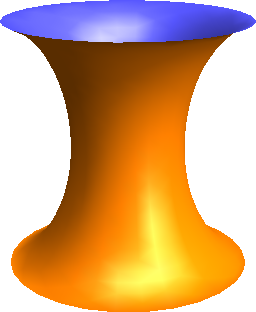
\includegraphics[scale=0.33333]{PortalSpace.png}
}
\subfigure[Part of a 2-black hole space]{
	\label{fig:second}
	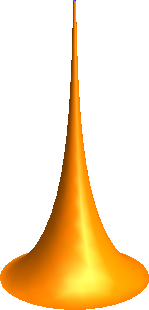
\includegraphics[scale=0.33333]{BlackHole.png}
}
\subfigure[Part of a 2-cone point space]{
	\label{fig:third}
	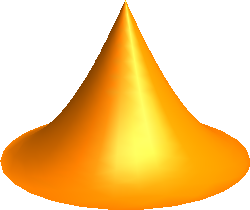
\includegraphics[scale=0.33333]{ConePoint.png}
}
\subfigure[Part of a 2-extended sphere]{
	\label{fig:fourth}
	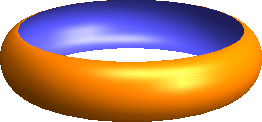
\includegraphics[scale=0.33333]{OuterTorus.png}
}
\end{figure}

I also hope to implement $S^3$ and $S^2 \times \mathbb{E}$. I may also implement $\mathbb{H}^2 \times \mathbb{E}$, but it doesn't combine well with the wormhole, so it won't be as useful.


One obstacle will be finding geodesics between two given points when spaces are glued together. In the spaces I have chosen, it is not difficult to construct a geodesic between two given points. However, this does not apply to the compound spaces made by gluing them together.

I can easily construct a geodesic from a given point moving in a given direction. By repeatedly constructing such geodesics at set lengths and taking note of the distance they are from the target point, I can use Newton's method to solve numerically for the geodesic between two given points.

Alternately, I can build a raytracer. Rather than finding the direction each point is in from the camera, I will construct geodesics corresponding to each pixel in the camera, shooting rays to see what lies in that direction. This leads to problems with light sources, since I still need to find the angle and distance of the light source from the given point. I have found three possible solution:

\begin{itemize}

\item I can give every point the same lighting, regardless of position. This will likely be useful for debugging, but it results in no shading, which will make it less useful or interesting.

\item I can use the camera as the light source. In this case, the geodesic that passes between the camera and a given point is the one I used to find that point to begin with. The shading will be a function only of distance, unless Phong shading is used. It will look better, but it will still be very limited.

\item I can simple fire photons in various directions from the light sources, and use them to color objects they strike. Photons can be used to give effects that are otherwise impossible, such as diffuse interreflection, where an object is illuminated by light reflected off of another object, but they generally take a very long time to calculate.

\end{itemize}

There is another notable detail. In Euclidean geometry, lighting falls of inversely with the square of distance. This does not apply in general. Changing the direction and distance a photon is emitted by $\varepsilon\textbf{u}$ for some unit vector $\textbf{u}$ will change where it hits by $M\varepsilon\textbf{u} + O(\varepsilon^2)$ for some matrix $M$. The brightness is inversely proportional to $|\det(M)|$.

More accurately, given the list of all vectors $\textbf{v}_1, \textbf{v}_2, ...$ such that the photons moving in that direction for that distance hit the given point, the brightness at that point is proportional to $\sum\frac{1}{|\det(M_{\textbf{v}_i})|}$. This is because, in general, two points can be connected by more than one geodesic.

\end{document}
